% Template for Cogsci submission with R Markdown

% Stuff changed from original Markdown PLOS Template
\documentclass[10pt, letterpaper]{article}

\usepackage{cogsci}
\usepackage{pslatex}
\usepackage{float}
\usepackage{caption}

% amsmath package, useful for mathematical formulas
\usepackage{amsmath}

% amssymb package, useful for mathematical symbols
\usepackage{amssymb}

% hyperref package, useful for hyperlinks
\usepackage{hyperref}

% graphicx package, useful for including eps and pdf graphics
% include graphics with the command \includegraphics
\usepackage{graphicx}

% Sweave(-like)
\usepackage{fancyvrb}
\DefineVerbatimEnvironment{Sinput}{Verbatim}{fontshape=sl}
\DefineVerbatimEnvironment{Soutput}{Verbatim}{}
\DefineVerbatimEnvironment{Scode}{Verbatim}{fontshape=sl}
\newenvironment{Schunk}{}{}
\DefineVerbatimEnvironment{Code}{Verbatim}{}
\DefineVerbatimEnvironment{CodeInput}{Verbatim}{fontshape=sl}
\DefineVerbatimEnvironment{CodeOutput}{Verbatim}{}
\newenvironment{CodeChunk}{}{}

% cite package, to clean up citations in the main text. Do not remove.
\usepackage{apacite}

% KM added 1/4/18 to allow control of blind submission
\cogscifinalcopy

\usepackage{color}

% Use doublespacing - comment out for single spacing
%\usepackage{setspace}
%\doublespacing


% % Text layout
% \topmargin 0.0cm
% \oddsidemargin 0.5cm
% \evensidemargin 0.5cm
% \textwidth 16cm
% \textheight 21cm

\title{Exploring potential gender stereotypes in the distributional
semantics of child-directed speech}


\author{{\large \bf Benjamin E. deMayo (bdemayo@princeton.edu)} \\ Princeton University}

\newlength{\cslhangindent}
\setlength{\cslhangindent}{1.5em}
\newenvironment{CSLReferences}%
  {}%
  {\par}

\begin{document}

\maketitle

\begin{abstract}
Abstract: In three analyses, I explore whether gender stereotypes might
be present in the distributional semantics of the CHILDES corpus
(MacWhinney 2014), a large compendium of transcribed conversations
between caregivers and their children, by training 2 commonly-used word
embedding models on the corpus. In the first analysis, I show that word
vector representations generated by both models capture some information
about gender that is correlated with human judgements of the
genderedness of individual words. In the second analysis, I show that
this relationship is consistent in speech directed at both boys and
girls and across the developmental period spanned by the children in
CHILDES. In the third analysis, I examine whether specific stereotypical
associations with gender are detectable in the vector space
representation of the words.

\textbf{Keywords:}
Add your choice of indexing terms or keywords; kindly use a semi-colon;
between each term.
\end{abstract}

\hypertarget{introduction}{%
\section{Introduction}\label{introduction}}

Gender is a highly salient social category that develops within the
first few years of life and maintains its importance across the lifespan
(Ruble, Martin, \& Berenbaum, 2006). Gender stereotypes, which can be
thought of as characteristics that are believed to be true of a gender
category as a whole, have their origins in toddlerhood, but become more
rigid in the preschool years into middle childhood (Halim \& Ruble,
2010). How children form concepts of gender, as well as the stereotypes
that are linked to those concepts, has long been a subject of research,
with some researchers proposing that language input to children could
have a consequential impact on children's conceptualizations of gender
categories.

Broadly speaking, two theoretical approaches have attempted to explain
how language input to children might shape their gender concepts. One
approach has emphasized the communication of knowledge from adults to
children in a ``top-down'' fashion, in which children hear statements
that explicitly communicate information about groups, such as generic
statements (e.g., {``girls are good at reading''}; Gelman, Ware, \&
Kleinberg, 2010). Another approach, which I focus on here, emphasizes
how children could pick up on subtle cues about gender concepts and
stereotypes from the statistics of their language input in a
``bottom-up'' fashion. In other words, children could learn that words
corresponding to particular activities, traits, occupations, and other
characteristics are themselves gendered by virtue of the other words
with which they co-occur. This latter approach therefore shares an
intimate link with the computational linguistic subfield of
distributional semantics, which seeks to characterize how the meaning of
linguistic items is related to how those items are distributed in large
bodies of text.

Several studies have leveraged the tools of distributional semantics to
examine whether gender stereotypes are appreciable natural language
corpora; some of these studies focus specifically on language that would
likely be heard by children. The general strategy used by these studies
has involved taking large bodies of text (usually those with several
million tokens, though this has not always been the case Lewis,
Borkenhagen, Converse, Lupyan, \& Seidenberg, 2020) and using them to
train a word embedding models, which generate representations of
individual word types in a high-dimensional vector space based on each
word type's co-occurrence with other types. The key assumption in such a
strategy is that words that frequently co-occur will have similar
meanings. Once vector representations of words are obtained, cosine
distances between individual lexical items in the vector space are
calculated as a proxy of semantic similarity, allowing researchers to
examine whether words' vector representations show patterns of
similarity to other words that might be expected given prevalent
societal stereotypes (e.g., that the word ``doll'' is closer to the word
``girl'' than it is to the word ``boy''). This general analytic
framework has been used to argue that gender stereotypes are present in
the distributional structure of large bodies of naturalistic text,
including web-based corpora, children's books, and transcripts of films
and television shows (Caliskan, Bryson, \& Narayanan, 2017;
Charlesworth, Yang, Mann, Kurdi, \& Banaji, 2021; Lewis \& Lupyan,
2020).

In this work, I extend prior findings by examining the human-like
gender-stereotypical biases that might emerge in the vector
representations obtained from training word embedding models on a body
of child-directed speech. Specifically, I use transcripts between
caregivers and children between the ages of 1 and 3 years old from the
North American English corpora in the Child Language Data Exchange
System {[}CHILDES; MacWhinney (2009){]} and extract vector-space
semantic representations using 2 commonly-used word embedding models,
word2vec (Mikolov, Chen, Corrado, \& Dean, 2013) and GloVe (Pennington,
Socher, \& Manning, 2014).

\hypertarget{method}{%
\section{Method}\label{method}}

\hypertarget{data-preprocessing}{%
\subsection{Data preprocessing}\label{data-preprocessing}}

Child-directed language was sourced from all of the North American
English transcripts in the CHILDES corpus (MacWhinney, 2009).
Transcripts were obtained using the \texttt{childes-db} API, which
allows researchers to access transcript utterances in a tabular format
that includes metadata about each utterance, including its speaker's
role (parent, grandparent, child, etc.), the gender of the child in the
conversation, and the lemmatized ``stem'' of the utterance (Sanchez et
al., 2019). From this tabular data, the stems of utterances from
mothers, fathers, grandparents and adults were extracted and
concatenated to create the training data, which contained X
conversations from Y dyads including Z children, and was comprised of A
word tokens and B word types.

\hypertarget{word-embedding-model-training}{%
\subsection{Word embedding model
training}\label{word-embedding-model-training}}

Two common word embedding models were used to obtain vector-space
representations for words in CHILDES. The first was Word2Vec (Mikolov et
al., 2013), which uses a 2-layer neural network to predict a given word
in a sentence given its surrounding words (continuous bag of words
approach, CBOW) or vice versa (skip-gram approach) and derives
vector-space representations of each word based on the neural network
weights between the input layer and the single hidden layer of the
network. The second was GloVe (Pennington et al., 2014), an unsupervised
learning algorithm which takes as input a sparse matrix encoding the
co-occurrence frequency of each pair of lexical items in a corpus, and
which learns vector representations for these items, such that the inner
product between two vectors closely approximates a logarithmic
transformation of the probability that those two lexical items co-occur
in the text. For our purposes here, the two techniques have the same
goal of extracting vector representations of words that are semantically
meaningful, even though GloVe's learning strategy emphasizes
co-occurrence probability between pairs of words more than Word2Vec,
which centers more on the semantic contexts that words appear in. In the
following analyses, the context window of each word embedding model is
set to 5 words in both directions from a target word. Word
representations derived from GloVe are vectors in a X-dimensional space
and those from Word2Vec are in a Y-dimensional space.

\hypertarget{analyses}{%
\section{Analyses}\label{analyses}}

\hypertarget{analysis-1-broad-comparison-between-word2vec-and-glove}{%
\subsection{Analysis 1: Broad comparison between Word2Vec and
GloVe}\label{analysis-1-broad-comparison-between-word2vec-and-glove}}

The first set of analyses is meant a coarse indication of whether
Word2Vec and GloVe are capturing roughly similar semantic information
for words in the CHILDES corpus, particularly as it concerns individual
words' genderedness.

\hypertarget{analysis-1a-association-between-genderedness-of-word-representations-in-word2vec-and-glove}{%
\subsubsection{Analysis 1A: Association between genderedness of word
representations in Word2Vec and
GloVe}\label{analysis-1a-association-between-genderedness-of-word-representations-in-word2vec-and-glove}}

In Analysis 1A, I examine whether the genderedness of a word's
representation in Word2Vec is associated with the genderedness of a the
same word's GloVe vector representation. A word's \emph{genderedness} is
operationalized here as the average cosine distance between the word's
vector representation and the vector representations of each of a set of
``anchor words'' which correspond to the concept of ``boy'' or ``girl.''
More precisely, for a given word \(w\) and sets of anchor words \(G\)
and \(B\) for the concepts \emph{girl} and \emph{boy}, respectively:

\vspace{5 mm}

\(G = \{{\text{girl, woman, sister, she, her, daughter}}\}\)

\(B = \{{\text{boy, man, brother, he, him, son}}\}\)

\(s(w, G) = \text{mean}_{g \in G}(\text{cos}(\vec{w}, \vec{g}))\)

\(s(w, B) = \text{mean}_{b \in B}(\text{cos}(\vec{w}, \vec{b}))\)

\hypertarget{first-level-headings}{%
\section{First-Level Headings}\label{first-level-headings}}

First level headings should be in 12 point , initial caps, bold and
centered. Leave one line space above the heading and
1/4\textasciitilde line space below the heading.

\hypertarget{second-level-headings}{%
\subsection{Second-Level Headings}\label{second-level-headings}}

Second level headings should be 11 point , initial caps, bold, and flush
left. Leave one line space above the heading and 1/4\textasciitilde{}
line space below the heading.

\hypertarget{third-level-headings}{%
\subsubsection{Third-Level Headings}\label{third-level-headings}}

Third-level headings should be 10 point , initial caps, bold, and flush
left. Leave one line space above the heading, but no space after the
heading.

\hypertarget{formalities-footnotes-and-floats}{%
\section{Formalities, Footnotes, and
Floats}\label{formalities-footnotes-and-floats}}

Use standard APA citation format. Citations within the text should
include the author's last name and year. If the authors' names are
included in the sentence, place only the year in parentheses, as in
(1972), but otherwise place the entire reference in parentheses with the
authors and year separated by a comma (Newell \& Simon, 1972). List
multiple references alphabetically and separate them by semicolons
(Chalnick \& Billman, 1988; Newell \& Simon, 1972). Use the et.
al.~construction only after listing all the authors to a publication in
an earlier reference and for citations with four or more authors.

For more information on citations in RMarkdown, see
\textbf{\href{http://rmarkdown.rstudio.com/authoring_bibliographies_and_citations.html\#citations}{here}.}

\hypertarget{footnotes}{%
\subsection{Footnotes}\label{footnotes}}

Indicate footnotes with a number\footnote{Sample of the first
footnote.} in the text. Place the footnotes in 9 point type at the
bottom of the page on which they appear. Precede the footnote with a
horizontal rule.\footnote{Sample of the second footnote.} You can also
use markdown formatting to include footnotes using this
syntax.\footnote{Sample of a markdown footnote.}

\hypertarget{figures}{%
\subsection{Figures}\label{figures}}

All artwork must be very dark for purposes of reproduction and should
not be hand drawn. Number figures sequentially, placing the figure
number and caption, in 10 point, after the figure with one line space
above the caption and one line space below it. If necessary, leave extra
white space at the bottom of the page to avoid splitting the figure and
figure caption. You may float figures to the top or bottom of a column,
or set wide figures across both columns.

\hypertarget{two-column-images}{%
\subsection{Two-column images}\label{two-column-images}}

You can read local images using png package for example and plot it like
a regular plot using grid.raster from the grid package. With this method
you have full control of the size of your image. \textbf{Note: Image
must be in .png file format for the readPNG function to work.}

You might want to display a wide figure across both columns. To do this,
you change the \texttt{fig.env} chunk option to \texttt{figure*}. To
align the image in the center of the page, set \texttt{fig.align} option
to \texttt{center}. To format the width of your caption text, you set
the \texttt{num.cols.cap} option to \texttt{2}.

\begin{CodeChunk}
\begin{figure*}[h]

{\centering 
\includegraphics{figs/2-col-image-1} 

}

\caption[This image spans both columns]{This image spans both columns. And the caption text is limited to 0.8 of the width of the document.}\label{fig:2-col-image}
\end{figure*}
\end{CodeChunk}

\hypertarget{one-column-images}{%
\subsection{One-column images}\label{one-column-images}}

Single column is the default option, but if you want set it explicitly,
set \texttt{fig.env} to \texttt{figure}. Notice that the
\texttt{num.cols} option for the caption width is set to \texttt{1}.

\begin{CodeChunk}
\begin{figure}[H]

{\centering 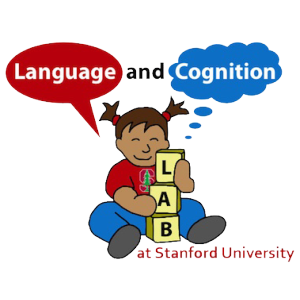
\includegraphics{figs/image-1} 

}

\caption[One column image]{One column image.}\label{fig:image}
\end{figure}
\end{CodeChunk}

\hypertarget{r-plots}{%
\subsection{R Plots}\label{r-plots}}

You can use R chunks directly to plot graphs. And you can use latex
floats in the fig.pos chunk option to have more control over the
location of your plot on the page. For more information on latex
placement specifiers see
\textbf{\href{https://en.wikibooks.org/wiki/LaTeX/Floats,_Figures_and_Captions}{here}}

\begin{CodeChunk}
\begin{figure}[H]

{\centering 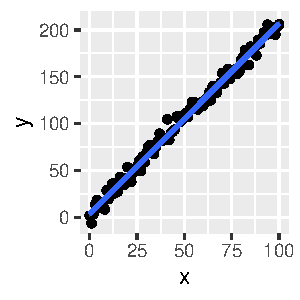
\includegraphics{figs/plot-1} 

}

\caption[R plot]{R plot}\label{fig:plot}
\end{figure}
\end{CodeChunk}

\hypertarget{tables}{%
\subsection{Tables}\label{tables}}

Number tables consecutively; place the table number and title (in 10
point) above the table with one line space above the caption and one
line space below it, as in Table 1. You may float tables to the top or
bottom of a column, set wide tables across both columns.

You can use the xtable function in the xtable package.

\begin{table}[H]
\centering
\begin{tabular}{rrrrr}
  \hline
 & Estimate & Std. Error & t value & Pr($>$$|$t$|$) \\ 
  \hline
(Intercept) & 0.09 & 0.11 & 0.8 & 0.43 \\ 
  x & 2.06 & 0.10 & 20.4 & 0.00 \\ 
   \hline
\end{tabular}
\caption{This table prints across one column.} 
\end{table}

\hypertarget{acknowledgements}{%
\section{Acknowledgements}\label{acknowledgements}}

Place acknowledgments (including funding information) in a section at
the end of the paper.

\hypertarget{references}{%
\section{References}\label{references}}

\setlength{\parindent}{-0.1in} 
\setlength{\leftskip}{0.125in}

\noindent

\hypertarget{refs}{}
\begin{CSLReferences}{1}{0}
\leavevmode\vadjust pre{\hypertarget{ref-caliskan2017semantics}{}}%
Caliskan, A., Bryson, J. J., \& Narayanan, A. (2017). Semantics derived
automatically from language corpora contain human-like biases.
\emph{Science}, \emph{356}(6334), 183--186.

\leavevmode\vadjust pre{\hypertarget{ref-ChalnickBillman1988a}{}}%
Chalnick, A., \& Billman, D. (1988). Unsupervised learning of
correlational structure. In \emph{Proceedings of the tenth annual
conference of the cognitive science society} (pp. 510--516). Hillsdale,
NJ: Lawrence Erlbaum Associates.

\leavevmode\vadjust pre{\hypertarget{ref-charlesworth2021gender}{}}%
Charlesworth, T. E., Yang, V., Mann, T. C., Kurdi, B., \& Banaji, M. R.
(2021). Gender stereotypes in natural language: Word embeddings show
robust consistency across child and adult language corpora of more than
65 million words. \emph{Psychological Science}, \emph{32}(2), 218--240.

\leavevmode\vadjust pre{\hypertarget{ref-gelman2010effects}{}}%
Gelman, S. A., Ware, E. A., \& Kleinberg, F. (2010). Effects of generic
language on category content and structure. \emph{Cognitive Psychology},
\emph{61}(3), 273--301.

\leavevmode\vadjust pre{\hypertarget{ref-halim2010gender}{}}%
Halim, M. L., \& Ruble, D. (2010). Gender identity and stereotyping in
early and middle childhood. In \emph{Handbook of gender research in
psychology} (pp. 495--525). Springer.

\leavevmode\vadjust pre{\hypertarget{ref-lewis2020might}{}}%
Lewis, M., Borkenhagen, M. C., Converse, E., Lupyan, G., \& Seidenberg,
M. S. (2020). What might books be teaching young children about gender?

\leavevmode\vadjust pre{\hypertarget{ref-lewis2020gender}{}}%
Lewis, M., \& Lupyan, G. (2020). Gender stereotypes are reflected in the
distributional structure of 25 languages. \emph{Nature Human Behaviour},
\emph{4}(10), 1021--1028.

\leavevmode\vadjust pre{\hypertarget{ref-macwhinney2009childes}{}}%
MacWhinney, B. (2009). The CHILDES project. \emph{Tools for Analyzing
Talk--Electronic Edition}, \emph{2}.

\leavevmode\vadjust pre{\hypertarget{ref-mikolov2013efficient}{}}%
Mikolov, T., Chen, K., Corrado, G., \& Dean, J. (2013). Efficient
estimation of word representations in vector space. \emph{arXiv Preprint
arXiv:1301.3781}.

\leavevmode\vadjust pre{\hypertarget{ref-NewellSimon1972a}{}}%
Newell, A., \& Simon, H. A. (1972). \emph{Human problem solving}.
Englewood Cliffs, NJ: Prentice-Hall.

\leavevmode\vadjust pre{\hypertarget{ref-pennington2014glove}{}}%
Pennington, J., Socher, R., \& Manning, C. D. (2014). GloVe: Global
vectors for word representation. In \emph{Empirical methods in natural
language processing (EMNLP)} (pp. 1532--1543). Retrieved from
\url{http://www.aclweb.org/anthology/D14-1162}

\leavevmode\vadjust pre{\hypertarget{ref-ruble2006gender}{}}%
Ruble, D. N., Martin, C. L., \& Berenbaum, S. A. (2006). Gender
development.

\leavevmode\vadjust pre{\hypertarget{ref-sanchez2019childes}{}}%
Sanchez, A., Meylan, S. C., Braginsky, M., MacDonald, K. E., Yurovsky,
D., \& Frank, M. C. (2019). Childes-db: A flexible and reproducible
interface to the child language data exchange system. \emph{Behavior
Research Methods}, \emph{51}(4), 1928--1941.

\end{CSLReferences}

\bibliographystyle{apacite}


\end{document}
